\section{Experiment}
\iffalse
https://github.com/HAIRLAB/Pre_Surv_COVID_19/

The choice of the cell is usually guided by the task at hand [J. Chung, C. Gulcehre, K. Cho, and Y. Bengio. Empirical evaluation of gated recurrent neural networks on sequence modeling.].
In all experiments we use an AE with 3 hidden layers, { D x , 30, D z , 30, D x } ; the number of neurons in the intermediate layers (30) has been set after preliminary experiments and is not a critical hyperparameter (comparable results were obtained using 20 or 40 neurons).
% In each experiment, we train the models for 5000 epochs with mini-batches containing 32 MTS using the Adam optimizer [kingma2014adam, D. Kingma and J. Ba. Adam: A method for stochastic optimization.] with an initial learning rate of 0.001.
% Data are in random order
% We consider the problem of classifying patients with and without surgical site infections from their blood samples.
% However, an important question for any autoencoder-style model is what prevents it from learning an identity mapping and effectively copying the input to the output. In that case all the information about the input would still be present but the representation will be no better than the input. There are two factors that control this behaviour. First, the fact that there are only a fixed number of hidden units makes it unlikely that the model can learn trivial mappings for arbitrary length input sequences.
% For this purpose, machine learning tools selected three biomarkers that predict the mortality of individual patients more than 10 days in advance with more than 90\% accuracy:

The problem was formulated as a classification task, where the inputs included basic information, symptoms, blood samples and the results of laboratory tests, including liver function, kidney function, coagulation function, electrolytes and inflammatory factors, taken from originally general, severe and critical patients (Table 1), as well as their associated outcomes corresponding to either survival or death at the end of the examination period. 
Medical records were collected by using standard case report forms that included epidemiological, demographic, clinical, laboratory and mortality outcome information (Table 2 and Supplementary Data 1).
The clinical outcomes were followed up to 24 February 2020.
% The medical information of all patients collected between 10 January and 18 February 2020 were used for model development.
Of the 375 cases included in the subsequent analysis, 201 recovered from COVID-19 and were discharged from the hospital, while the remaining 174 died> deceased.
% The performance models were evaluated by assessing the classification accuracy (ratio of true predictions over all predictions), the precision, sensitivity/recall and F1 scores (defined below): Definition of metrics with TP FP TN FN.

Selecting how deeper the model should be is another aspect of hyperparameter optimisation which can generally go from a single layer to three to four-layer deep model architecture where a three-layer architecture is used mostly in complex learning tasks. 

Because of the rapid spread of the virus, there has been a sharp increase in the demand for medical resources required to support infected people. Despite the desperate efforts to contain the disease and slow down its spread, many countries have been suffering from the shortage of hospital beds and critical care equipment for the timely treatment of ill patients[Ranney, M. L., Griffeth, V. & Jha, A. K. Critical supply shortages—The need for ventilators and personal protective equipment during the Covid-19 pandemic.,Gondi, S. et al. Personal protective equipment needs in the USA during the COVID-19 pandemic., Smereka, J. & Szarpak, L. The use of personal protective equipment in the COVID-19 pandemic era.]. Therefore, in addition to efficient diagnosis and treatment, accurate prognosis prediction is necessary to reduce the strain on healthcare systems and provide the best possible care for patients. When allocating limited medical resources, prediction models that estimate the risk of a poor outcome in an infected individual based on pre-diagnosis information could help to effectively triage patients.

In order to study the important blood biomarkers for predicting disease mortality, a retrospective study was conducted on 375 COVID- 19 positive patients admitted to Tongji Hospital (China) from January 10 to February 18, 2020. Demographic and clinical characteristics, and patient outcomes were investigated using machine learning tools to identify key biomarkers to predict the mortality of individual patient. A nomogram was developed for predicting the mortality risk among COVID-19 patients.

Yan et al. [21] reported a machine learning approach to select three biomarkers (lactic dehydrogenase (LDH), lymphocyte and high-sensitivity C-reactive protein (hs-CRP)) and using them to predict individual patients mortality, 10 days ahead with more than 90 percent accuracy. 
Blood samples collected between 10 January and 18 February, 2020 from 375 patients in Wuhan, China were retrospectively analyzed to identify reliable and relevant markers of mortality risk. Medical records were collected using standard case report forms, which included information on epidemiological, demographic, clinical, laboratory and mortality outcomes. Yan et al. [21] has published the dataset along with the article and the original study was approved by the Tongji Hospital Ethics Committee. Patients’ exclusion criteria for the study were: Age (<18 years), pregnant, breast- feeding and missing data (>20\%). Out of 375 patients, 187 (49.9\%) had fever while cough, fatigue, dyspnea, chest distress and muscular soreness were present in 52 (13.9\%), 14 (3.7\%), 8 (2.1\%), 7 (1.9\%) and 2 (0.5\%) patients respectively.
Of the 375 patients, 174 (46.4\) died, while 201 (53.6\%) patients recovered from COVID-19 and were discharged from hospital. Figure 1 summarizes the outcome of patients based on their initial conditions: general (197), severe (27) and critical (151). The minimal, maximal and median follow-up times (from hospital admission to death or discharge) for all 375 patients are 0 days, 35 days and 12 days, respectively.
Table 1 summarizes the demographic characteristics, clinical characteristics, and clinical outcomes of the subjects in the death and survival groups. There were 142 (37.9\%) patients, who were Wuhan residents, 2 (0.5\%) had contact with confirmed or suspected patients, 24 (6.4\%) were from familial cluster, 7 (1.9\%) were health workers, 2 (0.5\%) had contact with Huanan Seafood Market and 198 (52.5\%) had no contact history.

The main problem of neural networks, and therefore also of LSTMs, is the fact that is not always easy to understand how the network can identify the relationship between the input data and the target class.

LSTM-SA vs. reference models
The number of network nodes of the encoder and decoder are [128, 64, 32] and [32, 64, 128], respectively.
\fi
%%%%%%%%%%%%%%%%%%%%%%%%%%%%%%%%%%%%%%%%%%%%%%%%%%%%%%%%%%%%%%%%%%%%%%%%%%%%%%%%%%%
%% Precision and Recall on what? on survival and death both?
% [We design experiments to accomplish the following objectives:]
% Experiment section is organized as follows:
% 1. Prediction Performance on Classification on mortality.
% 2. blah.
% Convergency graph where all k-th runs are in a single figure.

Our experiments consist of two parts: (1) we evaluate the prediction performance of the proposed model, and (2) we identify the biomarkers which are most predictive for mortality. We conduct the experiments on two case studies from COVID-19 patients and intensive care unit (ICU) patients.

\subsection{Hyperparameters and Competitive Models}
We use the following hyperparameters of our semi-supervised autoencoder with a FCL or SVM classifier (SA-FCL, SA-SVM) found by the grid search. The accuracy on the test set is used as a criterion for selecting hyperparameters. The decoder $\phi_D$ has 3 fully connected layers with 200, 140, 100 nodes with a leaky Rectified Linear Unit (leaky ReLU, alpha = 0.1). Here we found that the leaky ReLU largely improves the reconstruction performance of the decoder, as we presume that the time stamp is the most important input feature for the decoder and this can be emphasized more with leaky ReLU activation function in a range $(- \infty, \infty)$, than the other activation functions in a smaller range. The encoder $\phi_E$ has a LSTM network with 60 units (thus the dimensionality of enriched representation $d_z = 60$) and a hyperbolic tangent activation function. $\gamma_1$ and $\gamma_2$ in Eq.~\eqref{eq: objective} are set to 0.005 and 0.1. The FCL classifier has 3 fully connected layers. The first two (with 120 and 60 nodes respectively) utilize the leaky ReLU activation function while the third (20 nodes) uses the soft-max activation function. The SVM classifier first transforms the enriched representations into 400 random features approximating the Gaussian kernel $k(\mathbf{x}, \mathbf{y}) \approx e^{-\frac{(\mathbf{x} - \mathbf{y})^2}{2\gamma_k^2}}$. The scale factor $\gamma_k$ is set to 10.

To minimize the loss function in Eq.~\eqref{eq: objective}, we use the Adam optimizer~\cite{kingma2014adam} with a learning rate of 0.0003 and the other parameters kept at their default values. We do not use regularization or dropout techniques, as they have not shown to improve the performance. Our model is built with Python 3.7 and Keras~\cite{chollet2015keras} framework and was tested using MacOS with a 3.4 GHz Quad-Core Intel Core i5 CPU and 16 GB DDR4 Ram. It took 2 and 9 hours to train the proposed model with 375 COVID-19 patients (200 iterations) and 3997 ICU patients (70 iterations).
% Considering our loss function is defined differently depending on the existence of label of sample, we train our model with the sample by sample instead of batch of samples. We build our model with Python 3.7 and Keras~\cite{chollet2015keras} framework. We use MacOS with 3.4 GHz Quad-Core Intel Core i5 CPU and 16 GB DDR4 Ram and it took 4 hours to train our model with 286 samples and 200 iterations.
% For prediction error, we have tried binary cross entropy and mean squared error, and mean squared error works better. Best Hyper-parameters are searched by following set of grid. Because RE\_DATE is important feature in decoder input, thus should be emphasized, we use leaky ReLU activation function at the input layer of decoder. And the prediction accuracy is improved with leaky ReLU at the input layer than tanh, while tanh works better in other layers.

For an ablation study to observe the effectiveness of our semi-supervised enrichment learning, we choose a supervised baseline LSTM (BLSTM) as a competing model by removing the decoders $\phi_{D}$ from our model SA-FCL. In addition to these longitudinal models, we use the following competitive models:
\begin{itemize}
    \item Deep Neural Network (DNN) of 5 fully connected layers with 150, 125, 100, 50, 25 nodes and ReLU activation function.
    \item Random Forest~\cite{ho1995random} (RF) with 34 max depth and 100 trees.
    \item Ridge Classifier (RC) with regularization parameter of 1.0.
    \item Support Vector Machine (SVM) with regularization parameter of 1.0 and radial basis kernel function.
\end{itemize}
Since these competitive models are not longitudinal models, we provide the concatenation of the most recent record $[\mathbf{x}_i^s, \mathbf{x}_i^{n_i}]$ to them. The training and test set are both provided to train SA in a semi-supervised manner, while only the training set is provided to train the other competing models. Although the order of participants is randomly shuffled to avoid the bias, we use the same training and test data across all the competing methods for a fair comparison.

\subsection{Predictions on Mortality of COVID-19 patients}

% Normalized, Min-max scaling. Time point to floating numbers, seconds after admission.
We conduct the classification task to predict the mortality of COVID-19 patients more than 10 days in advance and evaluate the performance of the predictive models.
We obtain the blood sample records (74 features), demographic information (age and gender), and associated mortality outcomes of 375 patients collected throughout their stay in Tongji hospital between January 10th and February 24th, 2020 following the previous research~\cite{yan2020interpretable}. We discard 17 samples where no time stamp was recorded. Among the remaining 358 samples, 192 patients survived and 166 patients died. The proportion of observed entries is 13.4\%. The order of samples is randomly shuffled to prevent bias. Each feature of the dataset is normalized by min-max scaling to the range [0, 1]. 
%% Simple LSTM is ablation study.
The outputs of the models are rounded up to the binary. We evaluate the predictive models with the following metrics:
\begin{equation}
\begin{aligned}
    &\text{Accuracy} = \frac{TP + TN}{TP + TN + FP + FN},\\
    &\text{Precision} = \frac{TP}{TP + FP},\\
    &\text{Recall} = \frac{TP}{TP + FN},\\
    &\text{F}_1\text{-score} = 2 \times \frac{\text{Precision} \times \text{Recall}}{\text{Precision} + \text{Recall}}.
\end{aligned}
\end{equation}
Since the precision and recall can be different when we predict fatality and survival respectively, we calculate and report the mean of the two cases. In table~\ref{tab: experimetal results COVID} and table~\ref{tab: experimetal results on ICU patients}, the average and standard deviation of the metrics across $k$ subgroups are reported following a $k$-fold cross validation scheme. $k$ is set to 4 (the size of test set is 25\% or 75\% of the studied cohort) or 5 (the size of test set is 20\% or 80\% of the studied cohort).
% SA, BLSTM, DNN, LASSO, RR, SVM denote the Semi-supervised BLSTM Auto Encoder (our model), Long Short Term Memory, Multi Layer Perceptron, Least Absolute Shrinkage and Selection Operator, Ridge Classifier, Support Vector Machine, respectively.
% From the 75 dynamic features from blood samples, and 4 static features from patient's demographic, we predict the patient's mortality in 10 days.
% \begin{table*}[h]
%     % \footnotesize
%     %\scriptsize
%     % \small
%     \setlength{\tabcolsep}{4pt} %% change column-wise separation.
%     \centering
%     \caption{The prediction performance of SA and the competitive models from k-fold cross validation. The best prediction is denoted as bold font.}\label{tab: experimetal results}
%     \begin{tabular}{|c|c|c|c|c|c|} %% 6 columns table
%     \hline
%     {\bfseries Test Set Size} & {\bfseries Model} & \multicolumn{1}{c}{{\bfseries Accuracy}} & \multicolumn{1}{c}{{\bfseries Precision}} & \multicolumn{1}{c}{{\bfseries Recall}} & {\bfseries $\text{F}_1$-score}\\ %% Headers
%     \Xhline{1pt}
%     \multirow{6}{*}{20\%} %% 6 rows group.
%     & SA & \multicolumn{1}{c}{{\bfseries 94.14$\pm$2.31}} & \multicolumn{1}{c}{\bfseries{93.35$\pm$2.45}} & \multicolumn{1}{c}{{\bfseries 93.15$\pm$2.84}} & {\bfseries 93.48$\pm$1.21}\\
%     & BLSTM & \multicolumn{1}{c}{92.56$\pm$3.24} & \multicolumn{1}{c}{91.11$\pm$1.45} & \multicolumn{1}{c}{92.45$\pm$8.12} & 91.43$\pm$5.40\\
%     & DNN & \multicolumn{1}{c}{80.63$\pm$11.52} & \multicolumn{1}{c}{76.58$\pm$10.94} & \multicolumn{1}{c}{83.80$\pm$11.97} & 80.02$\pm$11.14\\
%     & RF & \multicolumn{1}{c}{83.25$\pm$11.89} & \multicolumn{1}{c}{78.03$\pm$11.15} & \multicolumn{1}{c}{88.77$\pm$12.68} & 83.05$\pm$11.86\\
%     & RR & \multicolumn{1}{c}{79.32$\pm$11.33} & \multicolumn{1}{c}{76.76$\pm$10.97} & \multicolumn{1}{c}{79.54$\pm$11.36} & 78.12$\pm$11.16\\
%     & SVM & \multicolumn{1}{c}{79.32$\pm$11.33} & \multicolumn{1}{c}{77.55$\pm$11.08} & \multicolumn{1}{c}{78.12$\pm$11.16} & 77.83$\pm$11.11\\
%     \Xhline{1pt}
%     \multirow{6}{*}{25\%} %% 6 rows group.
%     & SA & \multicolumn{1}{c}{{\bfseries 92.47$\pm$3.43}} & \multicolumn{1}{c}{{\bfseries 91.84$\pm$8.41}} & \multicolumn{1}{c}{{\bfseries 91.97$\pm$2.34}} & {\bfseries 91.63$\pm$3.94}\\
%     & BLSTM & \multicolumn{1}{c}{91.91$\pm$3.69} & \multicolumn{1}{c}{91.38$\pm$8.94} & \multicolumn{1}{c}{91.62$\pm$1.89} & 91.17$\pm$3.98\\
%     & DNN & \multicolumn{1}{c}{81.90$\pm$11.70} & \multicolumn{1}{c}{79.25$\pm$11.32} & \multicolumn{1}{c}{82.92$\pm$11.85} & 81.05$\pm$11.58\\
%     & RF & \multicolumn{1}{c}{83.30$\pm$11.9} & \multicolumn{1}{c}{78.94$\pm$11.28} & \multicolumn{1}{c}{87.45$\pm$12.49} & 82.98$\pm$11.85\\
%     & RR & \multicolumn{1}{c}{80.50$\pm$11.50} & \multicolumn{1}{c}{81.13$\pm$11.16} & \multicolumn{1}{c}{76.14$\pm$10.88} & 78.56$\pm$11.22\\
%     & SVM & \multicolumn{1}{c}{80.50$\pm$8.12} & \multicolumn{1}{c}{80.11$\pm$11.45} & \multicolumn{1}{c}{77.65$\pm$11.09} & 78.86$\pm$11.27\\
%     \Xhline{1pt}
%     \multirow{6}{*}{75\%} %% 6 rows group.
%     & SA & \multicolumn{1}{c}{{\bfseries 89.48$\pm$1.59}} & \multicolumn{1}{c}{{\bfseries 88.59$\pm$2.27}} & \multicolumn{1}{c}{88.72$\pm$6.09} & {\bfseries 88.46$\pm$2.1}\\
%     & BLSTM & \multicolumn{1}{c}{87.91$\pm$1.07} & \multicolumn{1}{c}{87.41$\pm$3.22} & \multicolumn{1}{c}{86.07$\pm$4.59} & 86.57$\pm$1.4\\
%     & DNN & \multicolumn{1}{c}{80.09$\pm$11.44} & \multicolumn{1}{c}{74.94$\pm$10.71} & \multicolumn{1}{c}{86.86$\pm$12.41} & 80.46$\pm$11.50\\
%     & RF & \multicolumn{1}{c}{88.52$\pm$12.65} & \multicolumn{1}{c}{85.49$\pm$12.21} & \multicolumn{1}{c}{{\bfseries 91.32$\pm$13.0}} & 88.31$\pm$12.62\\
%     & RR & \multicolumn{1}{c}{79.03$\pm$11.29} & \multicolumn{1}{c}{75.54$\pm$10.79} & \multicolumn{1}{c}{82.41$\pm$11.77} & 78.82$\pm$11.26\\
%     & SVM & \multicolumn{1}{c}{77.98$\pm$11.11} & \multicolumn{1}{c}{75.06$\pm$10.7} & \multicolumn{1}{c}{80.18$\pm$11.45} & 77.54$\pm$11.08\\
%     \Xhline{1pt}
%     \multirow{6}{*}{80\%} %% 6 rows group.
%     & SA & \multicolumn{1}{c}{{\bfseries 88.06$\pm$1.07}} & \multicolumn{1}{c}{{\bfseries 86.98$\pm$1.82}} & \multicolumn{1}{c}{{\bfseries 87.03$\pm$3.29}} & {\bfseries 86.95$\pm$1.44}\\
%     & BLSTM & \multicolumn{1}{c}{84.07$\pm$5.55} & \multicolumn{1}{c}{86.55$\pm$2.91} & \multicolumn{1}{c}{77.60$\pm$16.00} & 80.66$\pm$9.94\\
%     & DNN & \multicolumn{1}{c}{79.46$\pm$11.35} & \multicolumn{1}{c}{72.80$\pm$10.40} & \multicolumn{1}{c}{82.19$\pm$11.17} & 77.21$\pm$11.03\\
%     & RF & \multicolumn{1}{c}{51.15$\pm$4.09} & \multicolumn{1}{c}{64.18$\pm$14.00} & \multicolumn{1}{c}{30.00$\pm$25.83} & 59.81$\pm$16.37\\
%     & RR & \multicolumn{1}{c}{78.14$\pm$11.16} & \multicolumn{1}{c}{70.78$\pm$10.11} & \multicolumn{1}{c}{82.19$\pm$11.17} & 76.06$\pm$10.87\\
%     & SVM & \multicolumn{1}{c}{74.16$\pm$10.79} & \multicolumn{1}{c}{66.22$\pm$9.46} & \multicolumn{1}{c}{79.03$\pm$11.3} & 72.06$\pm$10.29\\
%     \cline{1-6}
%     \end{tabular}
% \end{table*}

\begin{table}[h]
    \centering
    \scriptsize
    \caption{The prediction performance on COVID-19 patients. The best prediction is highlighted bold.}\label{tab: experimetal results COVID}
    \begin{tabular}{c c cccc}
        \toprule
        {\bfseries Test} & \multirow{2}{*}{{\bfseries Model}} & \multirow{2}{*}{{\bfseries Accuracy}} & \multirow{2}{*}{{\bfseries Precision}} & \multirow{2}{*}{{\bfseries Recall}} & \multirow{2}{*}{{\bfseries $\text{F}_1$-score}}  \\ {\bfseries Set} & & & & & \\
        \midrule
    \multirow{7}{*}{20\%}  
    & SA-FCL & \multicolumn{1}{c}{94.14$\pm$2.31} & \multicolumn{1}{c}{93.35$\pm$2.45} & \multicolumn{1}{c}{93.15$\pm$2.84} & 93.48$\pm$1.21\\
    & SA-SVM & \multicolumn{1}{c}{{\bfseries 94.15$\pm$1.21}} & \multicolumn{1}{c}{\bfseries{94.11$\pm$1.18}} & \multicolumn{1}{c}{{\bfseries 94.69$\pm$1.38}} & {\bfseries 94.13$\pm$1.08}\\
    & BLSTM & \multicolumn{1}{c}{92.56$\pm$3.24} & \multicolumn{1}{c}{91.11$\pm$1.45} & \multicolumn{1}{c}{92.45$\pm$8.12} & 91.43$\pm$5.40\\
    & DNN & \multicolumn{1}{c}{80.63$\pm$11.52} & \multicolumn{1}{c}{76.58$\pm$10.94} & \multicolumn{1}{c}{83.80$\pm$11.97} & 80.02$\pm$11.14\\
    & RF & \multicolumn{1}{c}{83.25$\pm$11.89} & \multicolumn{1}{c}{78.03$\pm$11.15} & \multicolumn{1}{c}{88.77$\pm$12.68} & 83.05$\pm$11.86\\
    & RC & \multicolumn{1}{c}{79.32$\pm$11.33} & \multicolumn{1}{c}{76.76$\pm$10.97} & \multicolumn{1}{c}{79.54$\pm$11.36} & 78.12$\pm$11.16\\
    & SVM & \multicolumn{1}{c}{79.32$\pm$11.33} & \multicolumn{1}{c}{77.55$\pm$11.08} & \multicolumn{1}{c}{78.12$\pm$11.16} & 77.83$\pm$11.11\\
    \midrule
    \multirow{7}{*}{25\%}
    & SA-FCL & \multicolumn{1}{c}{92.47$\pm$3.43} & \multicolumn{1}{c}{91.84$\pm$8.41} & \multicolumn{1}{c}{91.97$\pm$2.34} & {91.63$\pm$3.94}\\
    & SA-SVM & \multicolumn{1}{c}{{\bfseries 92.69$\pm$3.02}} & \multicolumn{1}{c}{\bfseries{92.2$\pm$2.25}} & \multicolumn{1}{c}{{\bfseries 92.31$\pm$2.09}} & {\bfseries 92.15$\pm$1.54}\\
    & BLSTM & \multicolumn{1}{c}{91.91$\pm$3.69} & \multicolumn{1}{c}{91.38$\pm$8.94} & \multicolumn{1}{c}{91.62$\pm$1.89} & 91.17$\pm$3.98\\
    & DNN & \multicolumn{1}{c}{81.90$\pm$11.70} & \multicolumn{1}{c}{79.25$\pm$11.32} & \multicolumn{1}{c}{82.92$\pm$11.85} & 81.05$\pm$11.58\\
    & RF & \multicolumn{1}{c}{83.30$\pm$11.9} & \multicolumn{1}{c}{78.94$\pm$11.28} & \multicolumn{1}{c}{87.45$\pm$12.49} & 82.98$\pm$11.85\\
    & RC & \multicolumn{1}{c}{80.50$\pm$11.50} & \multicolumn{1}{c}{81.13$\pm$11.16} & \multicolumn{1}{c}{76.14$\pm$10.88} & 78.56$\pm$11.22\\
    & SVM & \multicolumn{1}{c}{80.50$\pm$8.12} & \multicolumn{1}{c}{80.11$\pm$11.45} & \multicolumn{1}{c}{77.65$\pm$11.09} & 78.86$\pm$11.27\\
    \midrule
    \multirow{7}{*}{75\%}
    & SA-FCL & \multicolumn{1}{c}{{\bfseries 89.48$\pm$1.59}} & \multicolumn{1}{c}{88.59$\pm$2.27} & \multicolumn{1}{c}{88.72$\pm$6.09} & {88.46$\pm$2.1}\\
    & SA-SVM & \multicolumn{1}{c}{89.36$\pm$1.28} & \multicolumn{1}{c}{{\bfseries 88.69$\pm$1.81}} & \multicolumn{1}{c}{89.04$\pm$3.15} & {\bfseries 88.62$\pm$1.94}\\
    & BLSTM & \multicolumn{1}{c}{87.91$\pm$1.07} & \multicolumn{1}{c}{87.41$\pm$3.22} & \multicolumn{1}{c}{86.07$\pm$4.59} & 86.57$\pm$1.4\\
    & DNN & \multicolumn{1}{c}{80.09$\pm$11.44} & \multicolumn{1}{c}{74.94$\pm$10.71} & \multicolumn{1}{c}{86.86$\pm$12.41} & 80.46$\pm$11.50\\
    & RF & \multicolumn{1}{c}{88.52$\pm$12.65} & \multicolumn{1}{c}{85.49$\pm$12.21} & \multicolumn{1}{c}{{\bfseries 91.32$\pm$13.0}} & 88.31$\pm$12.62\\
    & RC & \multicolumn{1}{c}{79.03$\pm$11.29} & \multicolumn{1}{c}{75.54$\pm$10.79} & \multicolumn{1}{c}{82.41$\pm$11.77} & 78.82$\pm$11.26\\
    & SVM & \multicolumn{1}{c}{77.98$\pm$11.11} & \multicolumn{1}{c}{75.06$\pm$10.7} & \multicolumn{1}{c}{80.18$\pm$11.45} & 77.54$\pm$11.08\\
    \midrule
    \multirow{7}{*}{80\%}
    & SA-FCL & \multicolumn{1}{c}{{\bfseries 88.06$\pm$1.07}} & \multicolumn{1}{c}{{\bfseries 86.98$\pm$1.69}} & \multicolumn{1}{c}{{\bfseries 87.03$\pm$3.18}} & {\bfseries 86.95$\pm$1.44}\\
    & SA-SVM & \multicolumn{1}{c}{87.35$\pm$1.25} & \multicolumn{1}{c}{85.04$\pm$1.82} & \multicolumn{1}{c}{86.03$\pm$3.29} & {85.49$\pm$1.95}\\
    & BLSTM & \multicolumn{1}{c}{84.07$\pm$5.55} & \multicolumn{1}{c}{86.55$\pm$2.91} & \multicolumn{1}{c}{77.60$\pm$16.00} & 80.66$\pm$9.94\\
    & DNN & \multicolumn{1}{c}{79.46$\pm$11.35} & \multicolumn{1}{c}{72.80$\pm$10.40} & \multicolumn{1}{c}{82.19$\pm$11.17} & 77.21$\pm$11.03\\
    & RF & \multicolumn{1}{c}{51.15$\pm$4.09} & \multicolumn{1}{c}{64.18$\pm$14.00} & \multicolumn{1}{c}{30.00$\pm$25.83} & 59.81$\pm$16.37\\
    & RC & \multicolumn{1}{c}{78.14$\pm$11.16} & \multicolumn{1}{c}{70.78$\pm$10.11} & \multicolumn{1}{c}{82.19$\pm$11.17} & 76.06$\pm$10.87\\
    & SVM & \multicolumn{1}{c}{74.16$\pm$10.79} & \multicolumn{1}{c}{66.22$\pm$9.46} & \multicolumn{1}{c}{79.03$\pm$11.3} & 72.06$\pm$10.29\\
        \bottomrule
    \end{tabular}
\end{table}

\begin{figure}[h]
    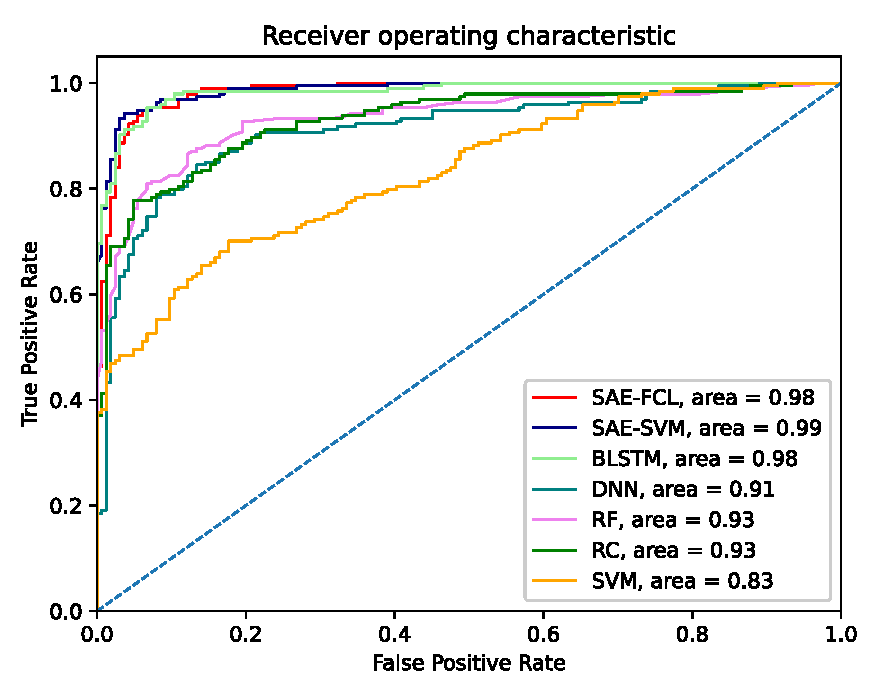
\includegraphics[width=1.0\linewidth]{figures/larger/roc_curve-covid-larger.eps}
    \caption{Receiver operating characteristic curves (ROC) and their area under the curve (AUC) of predictions on mortality of COVID-19 patients when proportion of test set is 20\%.} \label{fig: roc_curve COVID}
\end{figure}

In the experimental results in Table~\ref{tab: experimetal results COVID} and Fig.~\ref{fig: roc_curve COVID}, our model SA-FCL and SA-SVM are compared with the five competitive models. As shown by the results, our model outperforms the others for all different sizes of test sets. The performance gap between SA and the other competitive models even increases as the size of the test set grows. We suspect this is due to our semi-supervised learning approach that allows our model to learn from unlabeled samples while still fully utilizing the benefits of labeled samples. In addition, the predictions of the proposed model are more stable (with a smaller standard deviation) when compared to competing models. This gives our model increased flexibility and a competitive advantage in performance. This finding emphasizes the robustness of our model against large proportions of unlabeled samples, as well as its promise in early prediction of mortality.

\subsubsection{Classification Performance with Subset of Biomarkers}
The previous study~\cite{yan2020interpretable} has achieved the promising prediction performance on the mortality of COVID-19 patients with dataset same as ours. However, their model requires that the following biomarkers are measured: lactic dehydrogenase, lymphocyte and hight-sensitivity C-reactive protein. These three biomarkers have been identified as the mortality relevant biomarkers in their study, and the inclusion of these biomarkers may overly simplify the classification task. To further validate the usefulness of our model, we perform the classification task on the dataset whose those three biomarkers are excluded and inspect whether our model can still predict the mortality successfully. From the experimental results listed in Table~\ref{tab: experimetal results with the subset of biomarkers}, we have found that the proposed model shows acceptable prediction performance even if the three principle biomarkers are not given.
\begin{table}[h]
    \centering
    \caption{The prediction performance of SA-FCL when the subset biomarkers is given.}
    \begin{tabular}{ccccc}
    \toprule
    {\bfseries Test Set}  & {\bfseries Accuracy} & {\bfseries Precision} & {\bfseries Recall} & {\bfseries F$_1$-score} \\
    \midrule
    20\%  & 91.07$\pm$2.04  & 91.27$\pm$1.63  &89.18$\pm$4.65  &90.09$\pm$1.95  \\
    25\%  & 89.37$\pm$3.06  & 89.26$\pm$6.55  &88.07$\pm$2.99  &88.48$\pm$3.24  \\
    75\%  & 87.81$\pm$1.94  & 87.30$\pm$5.06  &86.83$\pm$6.72  &86.68$\pm$2.24  \\
    80\%  & 86.80$\pm$1.81  & 84.36$\pm$4.91  &87.70$\pm$2.17  &85.65$\pm$2.27  \\
    \bottomrule
    \end{tabular}
    \label{tab: experimetal results with the subset of biomarkers}
\end{table}

\subsubsection{Risk Factors of Mortality of COVID-19 patients}
It is vital to identify the mortality relevant biomarkers to predict the course of disease at diagnosis. We identify the risk factors from the blood sample measures of COVID-19 patients. Despite the high performance of deep learning models, their outputs are notoriously difficult to interpret. To identify which biomarkers (features) largely affect to the predictions, we add the perturbation to the input data and observe the changes in prediction.

For each $q$-th biomarker ($1 \leq q \leq D_l$) and $i$-th patient, we sample the column vector of perturbation $\mathbf{p}_{i,q} \in \Re^{n_i}$ from the normal distribution $\mathcal{N}(0, \sigma_q^2)$ with zero mean and the same standard deviation $\sigma_q$ as the observed distribution of the $q$-th biomarker across all $n_i$ time points and $n$ patients, and then perturb the measurement of $q$-th biomarker as follows:
\begin{equation}
\begin{aligned}
    &N_q = \sum_{i=1}^n \sum_{j=1}^{n_i} m^j_{i,q},\ \mu_q = \frac{1}{N_q}\sum_{i=1}^n \sum_{j=1}^{n_i} m_{i,q}^j \cdot x_{i,q}^j,\\
    &\sigma_q^2 = \frac{1}{N_q}\sum_{i=1}^n \sum_{j=1}^{n_i} m_{i,q}^j(x_{i,q}^j - \mu_q)^2,
\end{aligned}
\end{equation}
where $x_{i,q}^j$ and $m_{i,q}^j$ denote a measurement of $j$-th time step and $q$-th biomarker of $\mathbf{X}_i$ and $\mathbf{M}_i$.
Then the records whose $m$-th biomarker is perturbed and it's prediction change is:
\begin{equation}
\begin{aligned}
    &\mathbf{X}_i' = [\mathbf{x}_{i, 1}, \mathbf{x}_{i, 2}, \cdots, \mathbf{x}_{i, q} + \mathbf{p}_{i, q}, \cdots, \mathbf{x}_{i, D_l}],\\
    &\Delta\tilde{\mathbf{y}}_i = \| \phi_P(\phi_E(\mathbf{X}_i, \mathbf{M}_i, \mathbf{t}_i; \mathbf{\theta}_E), \mathbf{x}_i^s; \mathbf{\theta}_P)\\
    &- \phi_P(\phi_E(\mathbf{X}_i', \mathbf{M}_i, \mathbf{t}_i; \mathbf{\theta}_E), \mathbf{x}_i^s; \mathbf{\theta}_P) \|,
\end{aligned}
\end{equation}
where $\mathbf{x}_{i, q} \in \Re^{n_i}$ is the column vector of biomarker measurements of $i$-th patient collected across all the time points. Then the relative importance of the $q$-th biomarker is defined as the average of prediction changes over the all samples: $\frac{1}{n}\sum_{i=1}^n (\Delta\tilde{\mathbf{y}}_i / \sum_{j=1}^{n_i} m_{i,q}^j)$. By dividing the changes in predictions by the number of observations $\sum_{j=1}^{n_i} m_{i,q}^j$, we can prevent feature importance from being exaggerated by the large number of observations. We plot top 15 risk factors of mortality in Fig.~\ref{fig: identified-features COVID}.

\begin{figure}[h]
    \raggedright
    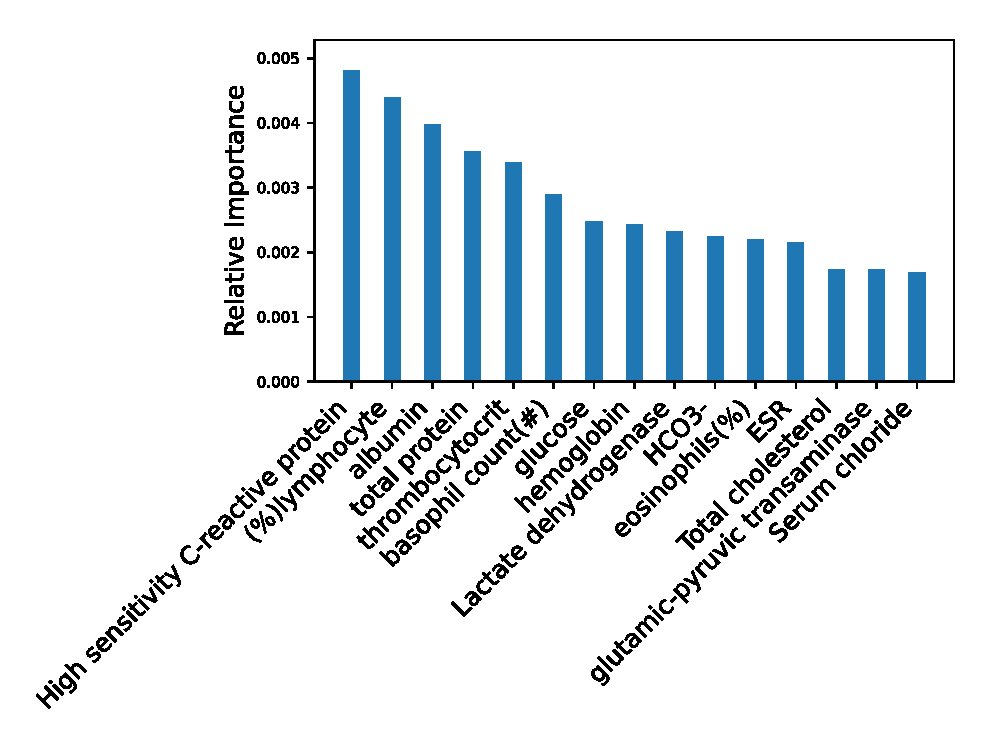
\includegraphics[width=1.0\linewidth]{figures/identified-features.eps}
    \caption{Top 15 important biomarkers in blood samples of COVID-19 patients.} \label{fig: identified-features COVID}
\end{figure}
The identified biomarkers have been shown in the literature to be related to the mortality of COVID-19 patients. For example, lactic dehydrogenase (LDH), lymphocyte and high-sensitivity C-reactive protein (hs-CRP) are the top 3 biomarkers relevant with the mortality of COVID-19 patients, identified by the XGBoost model \cite{yan2020interpretable} and previous medical researches~\cite{kishaba2014staging,ridker2008rosuvastatin,wang2020clinical}. % 11, 12, 16 cited.
To be specific, the increase of LDH indicates tissue or cell destruction and this is the strong sign of tissue or cell damage~\cite{yan2020interpretable}. The activity of idiopathic pulmonary fibrosis can be detected by Serum LDH~\cite{kishaba2014staging}. The hs-CRP is the risk factor for the continuous inflammation~\cite{bajwa2009plasma} and poor prognosis in acute respiratory distress syndrome~\cite{kishaba2014staging,sharma2016aetiology}. The lymphocyte is the common risk factor of COVID-19 patients~\cite{chan2020familial}, and lymphocyte has relation with the decrease in CD4 and CD8 T cells~\cite{liu2020longitudinal}.
Albumin have been found to be independently associated with mortality, at the Cox regression analysis~\cite{violi2020albumin}. The basophil count is known to be the risk factor of mortality and organ injury in COVID-19 patients~\cite{li2020immune}. 
% Pure LSTM

% The experimental result in \ref{tab: experimetal results} shows 
% It is validation accuracy on test set, not a training set. Output layer of predictor uses sigmoid activation function, and round up the output to generate binary class.

% \subsection{Reconstruction}
% Loss value changes by whether label is given or not, but loss converges stably. : convergency graph.

%% Low standard devation and large test set -> The prediction is stable and robust.

%%% COVID-19 risk factors previous studies.
%% Neutrophil-to-lymphocyte : Neutrophil-to-lymphocyte ratio as an independent risk factor for mortality in hospitalized patients with COVID-19, Yuwei Liu.

\subsection{Prediction on Mortality of Intensive Care Unit Patients}
Since the COVID-19 pandemic started less than two years ago, large-scale data of COVID-19 patients have not yet been accumulated. To evaluate the prediction performance on a larger dataset, we have downloaded time series measurements from blood tests~(37 features), demographic information and in-hospital mortality of 4000 patients admitted to the Intensive Care Unit (ICU) from PhysioNet Challenge 2012~\cite{silva2012predicting} and discarded 3 patients of no record. The detailed description on this dataset can be found in PhysioNet~(https://physionet.org/content/challenge-2012/1.0.0/). Age, gender, height, and ICU type~(Coronary Care Unit, Cardiac Surgery Recovery Unit, Medical ICU, and Surgical ICU) are provided as static data. The proportion of observed entries is 18\%. The overall mortality rate is 13.9\% and prediction with this unbalanced dataset can be challenging. We use the same hyperparameters used in COVID-19 patients dataset, except the followings:
\begin{itemize}
    \item LSTM with 30 units, $\gamma_1=1e-7$, and $\gamma_2=10$ in SA-FCL, SA-SVM, and BLSTM.
    \item Deep Neural Network of 3 fully connected layers with 100, 50, 25 nodes and ReLU activation function.
    \item Random Forest with 20 max depth and 70 trees.
    \item Ridge Classifier with regularization parameter of 0.5.
\end{itemize}
% These experimental results suggest that the proposed model can be successfully applied to large-scale blood experimental datasets.

As shown in Table~\ref{tab: experimetal results on ICU patients} and Fig.~\ref{fig: roc_curve ICU}, the overall performances are decreased in all models compared to COVID-19 case study and we presume that this is because the target labels (mortality rate is 13.9\%) are unbalanced. However the proposed model SA outperforms the competing models especially when the proportion of labeled samples is small, and the performance gaps are larger when compared to the experimental results from COVID-19 patients cohort. We presume that this is because the proposed model focuses on learning how to enrich the records of major cases (survived patients) to minimize the reconstruction error. As a result, the enriched representation of minor cases (died patients) can be quite different compared to major cases, therefore the classifier detects this differences and the enrichment approach can further improve the prediction. These results show that the proposed model can be successfully applied to the unbalanced and larger dataset.
% The larger change in the fewer labeled samples -> the number of observations is smaller -> enrichment more
% Larger std -> Therefore, the classifier is unable to utilize the unlabeled data to improve the accuracy, resulting in an unstable performance. 

\begin{table}
    \centering
    \scriptsize
    \caption{The prediction performance on mortality of ICU patients. The best prediction is highlighted in bold.}\label{tab: experimetal results on ICU patients}
    \begin{tabular}{c c cccc}
        \toprule
        {\bfseries Test} & \multirow{2}{*}{{\bfseries Model}} & \multirow{2}{*}{{\bfseries Accuracy}} & \multirow{2}{*}{{\bfseries Precision}} & \multirow{2}{*}{{\bfseries Recall}} & \multirow{2}{*}{{\bfseries $\text{F}_1$-score}}  \\ {\bfseries Set} & & & & & \\
        \midrule
    \multirow{7}{*}{20\%}  
    & SA-FCL & \multicolumn{1}{c}{86.39$\pm$2.23} & \multicolumn{1}{c}{74.36$\pm$1.14} & \multicolumn{1}{c}{{\bfseries 61.69$\pm$1.37}} & {\bfseries 68.43$\pm$1.38}\\
    & SA-SVM & \multicolumn{1}{c}{{\bfseries 86.87$\pm$2.68}} & \multicolumn{1}{c}{\bfseries 77.45$\pm$1.05} & \multicolumn{1}{c}{59.14$\pm$1.26} & {68.06$\pm$1.16}\\
    & BLSTM & \multicolumn{1}{c}{78.95$\pm$4.75} & \multicolumn{1}{c}{74.51$\pm$3.64} & \multicolumn{1}{c}{54.92$\pm$2.86} & 61.42$\pm$2.71\\
    & DNN & \multicolumn{1}{c}{76.09$\pm$3.54} & \multicolumn{1}{c}{60.5$\pm$4.69} & \multicolumn{1}{c}{54.83$\pm$3.86} & 55.83$\pm$3.82\\
    & RF & \multicolumn{1}{c}{80.27$\pm$3.54} & \multicolumn{1}{c}{64.12$\pm$2.61} & \multicolumn{1}{c}{58.15$\pm$2.27} & 59.18$\pm$2.72\\
    & RC & \multicolumn{1}{c}{79.64$\pm$8.84} & \multicolumn{1}{c}{57.79$\pm$6.8} & \multicolumn{1}{c}{61.35$\pm$4.29} & 59.14$\pm$5.25\\
    & SVM & \multicolumn{1}{c}{50.17$\pm$9.33} & \multicolumn{1}{c}{50.22$\pm$7.64} & \multicolumn{1}{c}{55.11$\pm$9.64} & 51.76$\pm$8.24\\
    \midrule
    \multirow{7}{*}{25\%}
    & SA-FCL & \multicolumn{1}{c}{85.6$\pm$3.15} & \multicolumn{1}{c}{73.92$\pm$4.4} & \multicolumn{1}{c}{{\bfseries 60.5$\pm$2.47}} & {65.29$\pm$3.65}\\
    & SA-SVM & \multicolumn{1}{c}{{\bfseries 85.94$\pm$2.11}} & \multicolumn{1}{c}{{\bfseries 75.92$\pm$1.25}} & \multicolumn{1}{c}{59.5$\pm$1.35} & {\bfseries 65.91$\pm$2.17}\\
    & BLSTM & \multicolumn{1}{c}{74.42$\pm$3.69} & \multicolumn{1}{c}{70.45$\pm$5.2} & \multicolumn{1}{c}{51.6$\pm$2.1} & 59.19$\pm$3.34\\
    & DNN & \multicolumn{1}{c}{72.42$\pm$5.34} & \multicolumn{1}{c}{57.11$\pm$5.81} & \multicolumn{1}{c}{51.2$\pm$3.02} & 53.25$\pm$5.45\\
    & RF & \multicolumn{1}{c}{77.19$\pm$5.12} & \multicolumn{1}{c}{61.27$\pm$4.35} & \multicolumn{1}{c}{56.65$\pm$4.15} & 58.67$\pm$3.28\\
    & RC & \multicolumn{1}{c}{76.29$\pm$7.2} & \multicolumn{1}{c}{55.09$\pm$4.7} & \multicolumn{1}{c}{59.25$\pm$6.84} & 56.2$\pm$5.84\\
    & SVM & \multicolumn{1}{c}{48.2$\pm$5.45} & \multicolumn{1}{c}{49.87$\pm$4.84} & \multicolumn{1}{c}{53.64$\pm$5.88} & 50.08$\pm$5.94\\
    \midrule
    \multirow{6}{*}{75\%}
    & SA-FCL & \multicolumn{1}{c}{{\bfseries 83.09$\pm$2.94}} & \multicolumn{1}{c}{70.61$\pm$3.15} & \multicolumn{1}{c}{56.34$\pm$2.61} & {62.46$\pm$2.98}\\
    & SA-SVM & \multicolumn{1}{c}{82.56$\pm$1.28} & \multicolumn{1}{c}{{\bfseries 71.11$\pm$2.48}} & \multicolumn{1}{c}{{\bfseries 56.81$\pm$1.81}} & {\bfseries 62.81$\pm$1.73}\\
    & BLSTM & \multicolumn{1}{c}{69.13$\pm$3.25} & \multicolumn{1}{c}{67.19$\pm$4.85} & \multicolumn{1}{c}{47.15$\pm$6.61} & 50.38$\pm$5.59\\
    & DNN & \multicolumn{1}{c}{62.54$\pm$4.05} & \multicolumn{1}{c}{51.14$\pm$5.25} & \multicolumn{1}{c}{47.35$\pm$8.1} & 48.24$\pm$6.05\\
    & RF & \multicolumn{1}{c}{67.41$\pm$5.21} & \multicolumn{1}{c}{56.29$\pm$5.04} & \multicolumn{1}{c}{52.21$\pm$5.42} & 53.29$\pm$5.45\\
    & RC & \multicolumn{1}{c}{66.9$\pm$11.45} & \multicolumn{1}{c}{51.94$\pm$10.18} & \multicolumn{1}{c}{53.15$\pm$7.2} & 51.61$\pm$8.92\\
    & SVM & \multicolumn{1}{c}{46.15$\pm$4.8} & \multicolumn{1}{c}{45.7$\pm$5.25} & \multicolumn{1}{c}{49.65$\pm$3.8} & 46.34$\pm$4.15\\
    \midrule
    \multirow{6}{*}{80\%}
    & SA-FCL & \multicolumn{1}{c}{{\bfseries 82.08$\pm$3.41}} & \multicolumn{1}{c}{69.97$\pm$3.92} & \multicolumn{1}{c}{{\bfseries 56.08$\pm$2.61}} & {\bfseries 61.95$\pm$3.24}\\
    & SA-SVM & \multicolumn{1}{c}{81.82$\pm$2.89} & \multicolumn{1}{c}{{\bfseries 70.14$\pm$2.46}} & \multicolumn{1}{c}{55.91$\pm$1.93} & {61.13$\pm$2.19}\\
    & BLSTM & \multicolumn{1}{c}{68.91$\pm$5.19} & \multicolumn{1}{c}{68.34$\pm$4.11} & \multicolumn{1}{c}{47.04$\pm$8.85} & 55.14$\pm$6.53\\
    & DNN & \multicolumn{1}{c}{61.31$\pm$4.8} & \multicolumn{1}{c}{51.01$\pm$6.24} & \multicolumn{1}{c}{46.13$\pm$4.15} & 48.7$\pm$4.11\\
    & RF & \multicolumn{1}{c}{71.14$\pm$2.19} & \multicolumn{1}{c}{56.25$\pm$5.95} & \multicolumn{1}{c}{51.9$\pm$3.71} & 53.14$\pm$5.89\\
    & RC & \multicolumn{1}{c}{65.95$\pm$5.62} & \multicolumn{1}{c}{50.15$\pm$9.45} & \multicolumn{1}{c}{51.48$\pm$8.1} & 51.14$\pm$9.42\\
    & SVM & \multicolumn{1}{c}{45.25$\pm$4.19} & \multicolumn{1}{c}{44.3$\pm$5.85} & \multicolumn{1}{c}{48.65$\pm$4.15} & 45.24$\pm$5.91\\
        \bottomrule
    \end{tabular}
\end{table}

\begin{figure}[h]
    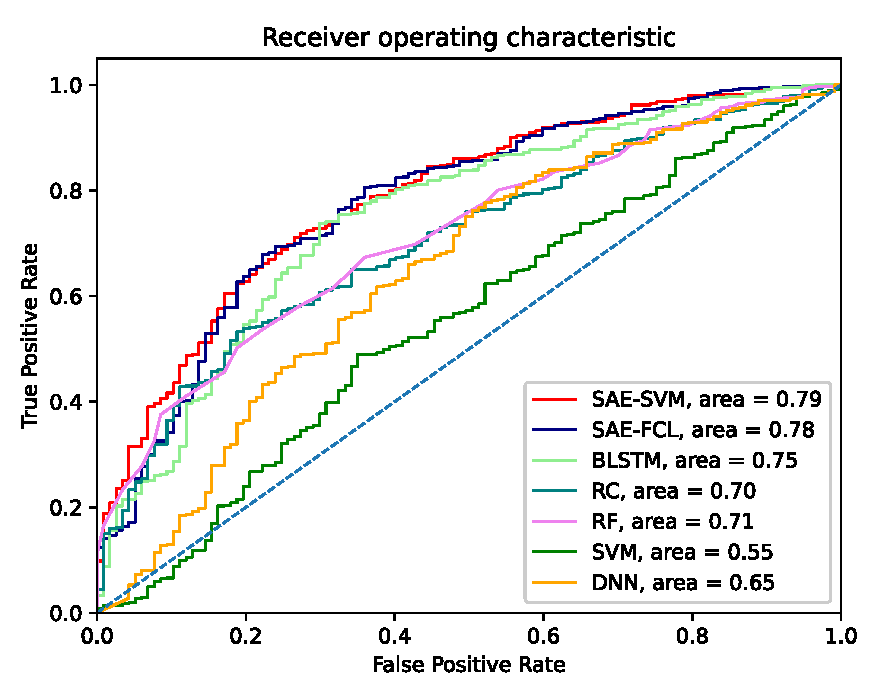
\includegraphics[width=1.0\linewidth]{figures/larger/roc_curve-icu-larger.eps}
    \caption{ROC and AUC of predictions on mortality of ICU patient when proportion of test set is 20\%.} \label{fig: roc_curve ICU}
\end{figure}

\subsubsection{Risk Factors of Mortality of ICU patients}
We also identify the most predictive biomarkers in mortality of ICU patients: Heart rate (HR), Invasive diastolic arterial blood pressure (DiasABP), and Non-invasive systolic arterial blood pressure (NISysABP). Based on the previous studies, heart rate is associated with the all-cause and cardiovascular mortality~\cite{zhang2016resting} and blood pressure control is important issue for minimizing the risk of mortality~\cite{wei2020optimal}. The low diastolic blood pressure is risk factor of mortality in systolic heart failure~\cite{javaheri2007central}. The biomarkers identified by our model in two case studies are in nice accordance with the previous studies, and provide the substantial evidence that our approach can identify the features associated with the prediction target.
\begin{figure}[h]
    \raggedright
    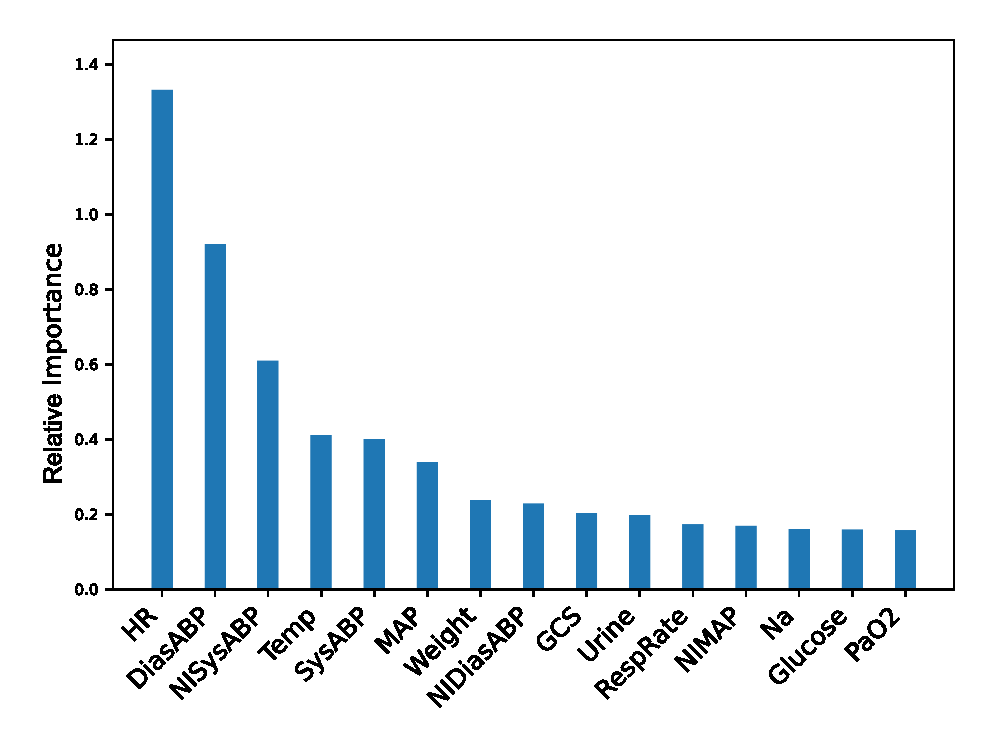
\includegraphics[width=1.0\linewidth]{figures/icu-biomarkers.eps}
    \caption{Top 15 important biomarkers in blood samples records of ICU patients.} \label{fig: identified-features ICU}
\end{figure}